\chapter{Pedestal Modeling and Theory}\label{ch:Modeling}

While a number of high-performance regimes (described in \cref{ch:HighPerformance}) have been established and are actively explored for tokamak operation, much of the physics governing these regimes is still unknown.  In particular, the physics underlying the structure of the pedestal is an area of active research, due in large part to the inherent difficulty in experimentally diagnosing the pedestal plasma as it varies over short scale lengths, and in the wide variability of H-mode behaviors observed in tokamak experiments.  Nevertheless confidence in the prediction of pedestal height and stability for ITER- and reactor-scale devices is essential: core temperature and pressure in the plasma are strongly sensitive to pedestal conditions due to profile stiffness driven by marginally-stable temperature-gradient modes \cite{Hubbard1998}\gnote{elaborate or reword}, thus fusion power density is controlled by the pressure pedestal structure.  Moreover, operation with large, uncontrolled Edge-Localized Modes (ELMs -- see \cref{sec:hcr_elmy}) can drive transient heat loads exceeding wall material tolerances on ITER-scale devices \cite{Loarte2003,Federici2003} -- an understanding of pedestal stability against ELMs is necessary for ITER operation and beyond.  This chapter provides a review of the efforts to date in theory and modeling of the pedestal, including the theoretical models used in the balance of this thesis.\nicesectionending\gnote{elaborate?}

\section{Early Models}\label{sec:mod_early}

\gnote{needs better title...}Initial efforts in understanding the pedestal took a variety of approaches, including models built from fairly simple \emph{ans\"{a}tze} for the physics determining the pedestal structure.  Several of these approaches are detailed here.  Overviews of these models may also be found in \cite[\S 2]{Hubbard2000,Hughes2005}.

\subsection{Empirical Observations}\label{subsec:mod_empirical}

Absent a firm understanding of the physics underlying the pedestal structure, experimental efforts have sought to characterize the pedestal in terms of simple scalings with engineering parameters.  The pedestal width, in particular, presented significant difficulty in this regard, as it tends to be quite robust, varying only over a narrow range on a given machine \cite{Maggi2010} -- observations on JET \cite{Breger1998} and Alcator C-Mod \cite{Hughes2002,Hughes2007a} found minimal variation of the pedestal width with plasma current or magnetic field, although a somewhat broader pedestal was observed at low current and with strong shaping on C-Mod \cite{Hughes2007,Hughes2007a}.  Accordingly, the measured gradients in density, temperature, and pressure in the steepest region of the pedestal trend linearly with the corresponding value at the pedestal top \cite{Breger1998,Hughes2007a}.

Multivariate dependences on engineering parameters may be explored with a reasonably general approach via power-law scalings, fitting pedestal data to scalings agnostic of any assumed underlying physics.  Suttrop \emph{et al.} \cite{Suttrop1997} found for ASDEX Upgrade pedestals

\begin{equation}
 \nabla p \sim B_T^{-0.31} \; P_{tot}^{0.16} \; \overline{n}_e^{-0.1} \; I_p^{2.1}
\end{equation}

\noindent A similar approach on C-Mod using an extensive dataset of EDA and ELM-free H-modes \cite{Hughes2002} found

\begin{equation}\label{eq:pedfits}
 \begin{aligned}
  n_{e,ped} &\sim I_p^{0.95} \; \overline{n}_{e,L}^{0.39} \; B_T^{-0.46}\\
  T_{e,ped} &\sim I_p^{0.95} \; \overline{n}_{e,L}^{-0.78} \; B_T^{0.80} \; P_{net}^{0.64}\\
  p_{e,ped} &\sim I_p^{1.98} \; \overline{n}_{e,L}^{-0.56} \; P_{net}^{0.48}
 \end{aligned}
\end{equation}

\noindent (here $\overline{n}_{e,L}$ is the L-mode target density, as pedestal density is not readily controllable in EDA H-mode).  However, later studies asserted that the magnetic-field dependence was overstated in the above \cite{Hughes2006}.  While these empirical models perform reasonably well on their respective experimental data, confident extrapolation to ITER-scale operation requires a physics-based understanding of the pedestal structure.

\subsection{Neutral Penetration \& the Density Pedestal}\label{subsec:mod_neutral}

Given the proximity of the plasma pedestal to neutral gas from fueling apparatus and wall outgassing in the edge, it is logical that the density profile should depend strongly on interaction with and ionization of neutral particles in the pedestal.  Based on a relatively simple particle transport model, the pedestal width is expected to scale with the characteristic neutral penetration length before ionization \cite{Hughes2005,Mahdavi2002}:

\begin{equation}\label{eq:neutralpenetration}
 \lambda_{neutral} = \frac{v_n}{n_e \langle \sigma v \rangle_{ion}}
\end{equation}

\noindent where $v_n$ is the velocity of neutrals entering the pedestal (set by the neutral thermal temperature in the edge) and $\langle \sigma v \rangle_{ion}$ is the velocity-averaged ionization cross-section.  Given that $v_n$ is independent of plasma conditions and that $\langle \sigma v \rangle_{ion}$ is consistent over the temperatures of interest in the edge \cite{Hughes2005}, therefore we expect the simple relation $\Delta_{n} \sim 1/n_{e,ped}$.  More complex models for the neutral penetration typically reproduce the dependence on $\lambda_{neutral}$.

However, experimental observations of the density pedestal conflict with these relatively simple predictions.    Observations in similarity experiments between DIII-D, JET, and ASDEX Upgrade \cite{Beurskens2011} were inconsistent with the simple model: although DIII-D data were consistent with the trends found in the model, data from JET were not, and moreover the model predicted an inconsistent scaling between the two machines for pedestal density and width.  Likewise, predictions based on pedestal widths set by neutral penetration performed poorly as a predictor for pedestal height in a multi-machine scaling from AUG, DIII-D, JT-60U, and JET \cite{Onjun2002}.  EDA H-modes on Alcator C-Mod show near-complete insensitivity of the density pedestal to neutral interactions -- the density pedestal instead saturates to a level dictated by plasma transport (predicted best by $n_{e,ped} \sim I_p$), with fueling via edge gas puffing having little effect on the density pedestal \cite{Hughes2006,Hughes2007}.

In addition to significant sensitivity to machine and discharge conditions and wall materials \cite{Beurskens2011}, density pedestal behavior appears to be strongly sensitive to magnetic configuration -- experiments on MAST \cite{Maggi2010} found that, while the density pedestal width was poloidally constant in single-null discharges, the density pedestal is measurably broader on the outboard, low-field side in double-null discharges.  These results indicate that plasma-neutral interactions in the density pedestal are quite complex, and dependent on poloidal transport behaviors and fueling asymmetries \cite{Maggi2010}.  This remains an important area of research, as ITER is expected to have an edge that is highly opaque to neutrals, complicating the density pedestal structure and fueling scenarios for high-density plasmas \cite{Hughes2007,Maggi2010}.

\subsection{Ion-Orbit Loss \& Gyroradius Models}\label{subsec:mod_ionorbitloss}

Due to the importance in the edge $E_r$ well in pedestal formation, modeling efforts naturally turned to potential sources for the electric field to explain the pedestal.  One suggested source was ion orbit loss across the last closed flux surface, in which the gyro-motion of ions near the edge intersect the SOL or the plasma-facing material surfaces -- the charge imbalance induced by this particle ``leak'' results in a radial electric field \cite{Shaing1990}.  Assuming ion orbit losses drive the $E_r$ well, the $\vec{E}\times\vec{B}$ shear layer width ought to be governed by the banana orbit width, which scales as the poloidal gyroradius $\rho_{i,pol} \sim \sqrt{T_i}/B_p$.  Accounting for the squeezing effect of the radial electric field on the banana orbit width, Shaing \cite{Shaing1992} gives for the well width

\begin{equation}\label{eq:Shaing_width}
 \begin{aligned}
  &\Delta_{\vec{E}\times\vec{B}} \propto \sqrt{\varepsilon} \frac{\rho_{i,pol}}{\sqrt{S}}\\
  &S = \left| 1 - \frac{1}{B_p \omega_{ci,p}} \frac{dE_r}{dr}\right|
 \end{aligned}
\end{equation}

\noindent where $S$ is the squeezing factor and $\omega_{ci,p}$ is the ion cyclotron frequency evaluated with the poloidal field.  The model is further refined by Itoh \& Itoh \cite{Itoh1996} to include the broadening effects of viscosity shear.  The predicted trend is observed in ELM-free H-modes on JT-60U \cite{Hatae1998}, with $\Delta \approx 3.3 \sqrt{\varepsilon} \rho_{i,pol}$; however, as the squeezing factor $S$ is estimated to be near-unity, the pedestal width is broader by a factor of $\sim 3.3$ than the $\sim \sqrt{\varepsilon} \rho_{i,pol}$ banana width.  ELMy H-modes on JT-60U exhibit a similar scaling at weak shaping, with a broader pedestal and additional safety factor dependence $\Delta \approx 5 \rho_{i,pol} q_{95}^{-0.3}$ at higher triangularity \cite{Kamada1999}.

However, other predictions and experimental observations contradict these results.  Depending on the calculation method of growth rate suppression by $\vec{E}\times\vec{B}$ sheared flow, the pedestal width may scale with the gyroradius anywhere from $\Delta \sim \left(\rho^*\right)^{1/2}$ to $\Delta \sim \rho^*$, where $\rho^*$ indicates the gyroradius normalized to the plasma minor radius \cite{Onjun2002,Beurskens2011}.  Alternately, stabilization of drift-ballooning modes leads to a predicted dependence of $\Delta \sim \rho_{i,pol}^{2/3}$ \cite{Wilson1997}; similarly, diamagnetic stabilization in the pedestal leads to the prediction of $\Delta \sim I_p^2 \rho_{i,pol}^{2/3}$ \cite{Rogers1999}.  Observations on DIII-D \cite{Osborne1998} found a dependence of $\Delta/R \sim (\rho_{i,pol}/R)^{0.67}$, while observations on ASDEX Upgrade \cite{Beurskens2011,Suttrop2000a} found no gyroradius dependence for the pedestal width.

Distinguishing between these scalings is difficult given the diagnostic complications inherent in pedestal measurements, and the narrow range over which $\rho_i$ or the pedestal and $E_r$ well width vary on a given machine \cite{Gohil1998,Maggi2010}.  Moreover, alternate models propose a scaling with poloidal beta at the pedestal top, rather than poloidal gyroradius, with trends of width of $\Delta \sim \beta_{p,ped}^{0.4}$ to $\sim \beta_{p,ped}^{0.5}$ observed on DIII-D \cite{Osborne1998,Groebner1998a}, JET \cite{Maggi2010}, JT=60U \cite{Urano2008}, and ASDEX Upgrade \cite{Beurskens2011}.  Due to the strong covariance between $\rho_{i,pol} \sim \sqrt{mT}/I_p$ and $\sqrt{\beta_{p,ped}} \sim \sqrt{nT}/I_p$ these trends are quite difficult to separate.  However, dedicated experiments to separate the two, either via pumping to vary density and temperature at fixed pressure, exploiting the density dependence in $\beta_{p,ped}$ \cite{Osborne1998}, or via isotope variation targeting the mass dependence in $\rho_{i,pol}$ \cite{Urano2008,Saibene1999}, found the $\beta_{p,ped}$ scaling to be the better predictor, with a weaker secondary gyroradius dependence $\Delta \sim \rho_{i,pol}^{0.2} \beta_{p,ped}^{0.5}$ \cite{Urano2008,Maggi2010}.  The physics underlying the $\Delta \sim \sqrt{\beta_{p,ped}}$ scaling will be discussed in detail in \cref{sec:mod_turbulence}.\nicesectionending

\section{MHD Stability: Peeling-Ballooning Modes}\label{sec:mod_pb}

Early observations of the pedestal in ELMy H-mode identified ballooning MHD instabilities as a possible driver for the ELM instability.  Numerous experiments identified a pressure-gradient effect tied to the ELM trigger \cite{Kamada1996}\gnote{pull other cites!}, with the value of the pressure gradient at the ELM trigger increased with plasma current and increased shaping consistent with ballooning MHD behavior \cite{Suttrop2000a}.

\subsection{Ballooning MHD}\label{subsec:mod_balloon}

\begin{itemize}
 \item EDA H-mode modeled to be ideal-ballooning stable; P-B only describes ELMy H-mode \cite{Mossessian2002}
 \item increased triangularity reduces $\nabla p$, $n_{e,ped}$ in EDA; contrast with ELMy, where shape stabilizes P-B modes, seems to destabilize QCM earlier in EDA \cite{Hughes2007a}
\end{itemize}

\subsection{Peeling MHD}\label{subsec:mod_peel}

\subsection{ELITE Code}\label{subsec:mod_elite}

\begin{itemize}
 \item strong shaping impacts stability contour in $j-\alpha_{MHD}$ space \cite{Snyder2009}
 \item collisionality $\rightarrow$ bootstrap current $\rightarrow$ magnetic shear in edge sets where in stability contour pedestal hits \cite{Snyder2009}
 \item due to interplay, nonlocal effects between shaping, collisionality, rotation, shafranov shift, safety factor, must calculate P-B stability in 2D: can't reduce to scalar parametrization \cite{Snyder2009}
 \item Snyder2009 refs Huysmans2005, Turnbull2003, Medvedev2006 \cite{Huysmans2005,Turnbull2003,Medvedev2006} for reviews of alternate MHD codes
 \item RMP approaches P-B boundary, EDA, type-III ELMs P-B stable, grassy/type-II ELMs near boundary, QH near low-$n$ peeling side -- P-B boundary figure of merit in general for H-mode pedestal \cite{Snyder2009}
\end{itemize}

\begin{figure}
 \pushtooutside
 \fcapside[60mm]{\caption[Schematic of peeling-ballooning MHD stability space.]{Schematic of the stability space to coupled peeling-ballooning MHD modes, set by the edge pressure gradient and current density.  Ballooning modes are driven by pressure gradient but stabilized by magnetic shear driven by edge currents, while kink/peeling modes are current-driven but stabilized by pressure gradients.  \note{Ref to Snyder?}}\label{fig:mod_pbcartoon}}{\includegraphics[width=100mm]{graphics/ModelingTheory/pbcartoon.pdf}}
\end{figure}

\nicesectionending

\section{Kinetic-Ballooning Turbulence Modeling}\label{sec:mod_turbulence}

\nicesectionending

\section{The EPED Model}\label{sec:mod_eped}

In light of the importance of the pedestal structure for optimized fusion performance -- both by maximizing fusion power density via the pressure pedestal height constraint on core profiles \cite{Kinsey2011}, and by avoiding or mitigating large, damaging ELMs \cite{Loarte2003,Federici2003} -- a predictive understanding of the pedestal is highly desirable for planned operations on ITER and beyond.  Models based on peeling-ballooning MHD instability, particularly the ELITE code (\cref{subsec:mod_elite}), have proven quite successful at capturing the limiting physics of the ELMy H-mode pedestal.  However, these calculations typically rely on experimental profiles and magnetic equilibria reconstructed after the fact, and as such cannot by themselves provide predictive capability.  Similarly, the constraint set by kinetic-ballooning mode (KBM) turbulence (\cref{sec:mod_turbulence}) corresponds well with pedestal observations in profiles with steep pressure gradients in the pedestal, but cannot by itself uniquely constrain the pedestal structure.  Here we introduce the EPED series of models \cite{Snyder2011}, which combines these two constraints into a single predictive model for the ELMy H-mode pedestal.

To incorporate predictive capability into the peeling-ballooning MHD stability model calculated by ELITE, the EPED model must characterize peeling-ballooning stability as accurately as possible using only parameters known prior to the plasma discharge, set by operator control; however, as discussed in \cref{subsec:mod_elite}, the inherent nonlocality of the problem still requires a 2-dimensional MHD calculation.  To that end, the model employs a set of model Miller equilibria \cite{Miller1998}, up/down-symmetric equilibria allowing for plasma elongation and triangularity defined with analytic plasma profiles such that the essential physics in the pedestal (namely, the pressure gradient and bootstrap current profiles) is nearly matched to experimental conditions \cite{Snyder2009}.  Using this setup, the model equilibria may be defined by a small set of scalar parameters: major and minor radius $R$ and $a$, elongation and shaping $\kappa$, $\delta$ (recall that in these up/down-symmetric equilibria $\delta_l = \delta_u = \delta$), plasma current $I_p$, and applied field $B_T$, set the magnetic equilibrium when combined with the target global normalized pressure (typically the Troyon normalized $\beta_N$ \cite{Troyon1984}).  Global beta also impacts the pedestal stability via the beneficial effect of increased Shafranov shift in the core on MHD stability\gnote{ref this in peeling-ballooning section!}.

\begin{figure}[ht]
 \pushtooutside
 \fcapside[60mm]{\caption[Illustration of the peeling-ballooning MHD and KBM constraints used in the EPED model.]{Illustration of the peeling-ballooning MHD and kinetic-ballooning turbulent constraints used in the EPED model.  The peeling-ballooning constraint, calculated by ELITE, results in a trend roughly of $p_{ped} \sim \Delta_\psi^{3/4}$, while the KBM width constraint calculated via the ballooning-critical pedestal (BCP) technique sets $p_{ped} \sim \Delta_\psi^{2}$.  The unique solution to these constraints is the EPED prediction for the pedestal width and height.  The prediction is here shown compared to the measured pedestal from DIII-D shot 132003 (reproduced from \cite{Snyder2011}) \note{get permission}}}{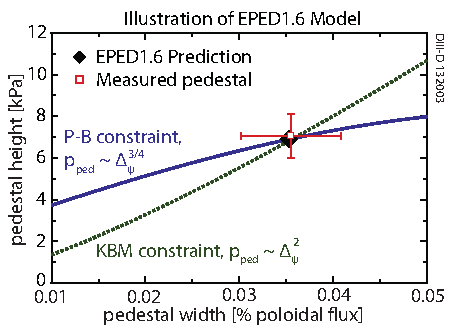
\includegraphics[width=100mm]{graphics/ModelingTheory/epedcartoon.pdf}}
\end{figure}

\begin{figure}[ht]
 \pushtooutside
 \fcapside[60mm]{\caption[EPED predictions versus measured pressure pedestal heights.]{EPED predictions versus measured pressure pedestal heights from DIII-D and C-Mod, spanning a significant range of pedestal pressures.  Notably, C-Mod pressure pedestals reach within a factor of $\sim 2$ of the predicted ITER pedestal height.  \note{ref to Hughes paper}}\label{fig:mod_epedpredictions}}{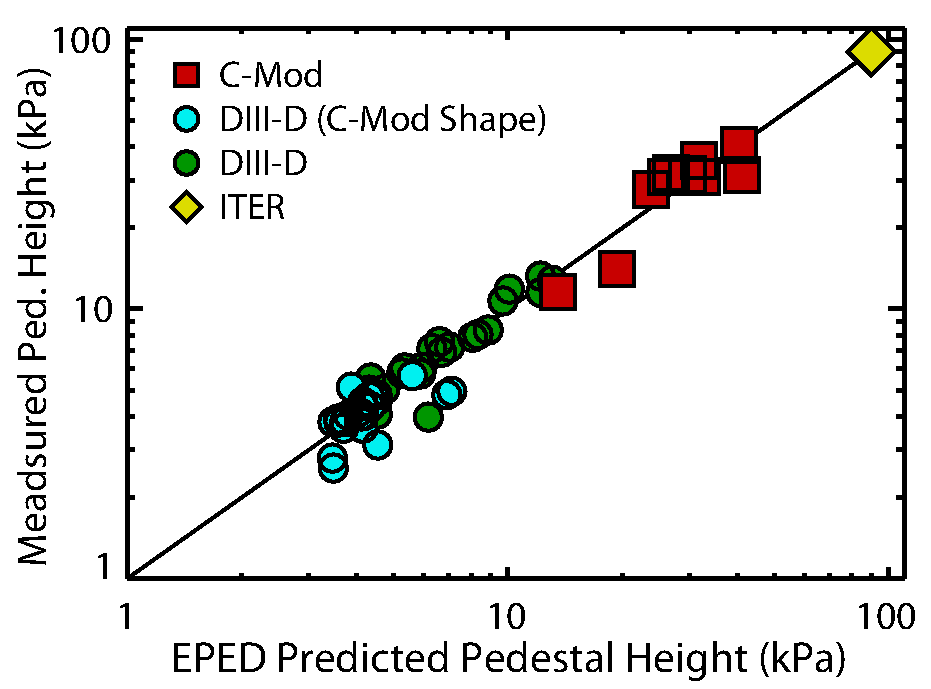
\includegraphics[width=100mm]{graphics/ModelingTheory/eped.pdf}}
\end{figure}

\begin{itemize}
 \item 
\end{itemize}

\nicechapterending

\bibliographystyle{../plainurl}
\bibliography{../references}